% Classe do documento e parâmetros gerais.
\documentclass[a4paper,openright,twoside,11pt]{report}

% Packages utilizadas e respetivos parâmetros.
\usepackage[utf8]{inputenc}
\usepackage[portuguese]{babel}
\addto{\captionsportuguese}{\renewcommand{\bibname}{Refer\^{e}ncias}}
\addto{\captionsportuguese}{\renewcommand{\contentsname}{\'{I}ndice}}
\addto{\captionsportuguese}{\renewcommand{\appendixname}{Ap\^{e}ndice}}

\usepackage{lipsum} % gerador de texto
\usepackage{graphicx}
\usepackage{url}
\usepackage[Algoritmo]{algorithm}
\usepackage{algorithmicx}
\usepackage{algpseudocode}
\renewcommand{\algorithmicrequire}{\textbf{Dados: }}
\renewcommand{\algorithmicensure}{\textbf{Resultado: }}

% Definições das dimensões das páginas
\setlength{\textheight}{24.00cm}
\setlength{\textwidth}{15.50cm}
\setlength{\topmargin}{0.35cm}
\setlength{\headheight}{0cm}
\setlength{\headsep}{0cm}
\setlength{\oddsidemargin}{0.25cm}
\setlength{\evensidemargin}{0.25cm}

%\renewcommand{\baselinestretch}{1}

% Página inicial (capa)
\title{
   \vspace{-50mm}
   \begin{minipage}[l]{\textwidth}
      \hspace{-20mm}\resizebox{75mm}{!}{
\includegraphics{./figures/logoISELnew2.png}}\\
   \end{minipage}\\[20mm]
   {\textbf{SecDash} \\ Dashboard de Vulnerabilidades de Segurança Multi-Repositório}
}

% Nome dos autores (um por linha)
\author{
      \begin{tabular}{c}
         Gonçalo Filipe Domingos Carvalho \\
         Rodrigo dos Ramos Pais Henriques Vitorino \\[50mm]
      \end{tabular}
}

\date{
\begin{tabular}{ll}
  {Orientador:} & Professor Doutor José Simão
\end{tabular}\\[10mm]
Relatório do projeto realizado no âmbito de Projecto e Seminário\\
Licenciatura em Engenharia Informática e de Computadores\\[20mm]
Junho de 2026}


\begin{document}
\pagenumbering{roman}
\thispagestyle{empty}
\maketitle

\baselineskip 18pt % line spacing: 12pt for single, 18pt for 1 1/2, and 24pt for double spacing

\newpage
\thispagestyle{empty}
% Fim da contracapa

% Página com identificação completa (número e nome) e assinaturas do(s) estudante(s) e do(s) orientador(es)
\cleardoublepage
\setcounter{page}{1}
\begin{center}
\textsc{\LARGE Instituto Superior de Engenharia de Lisboa}\\[50mm]

{\large \bf  SecDash}\\[20mm]

\begin{tabular}{rl}
	49219 & Gonçalo Filipe Domingos Carvalho \\[10mm]
	& \rule{75mm}{0.5pt} \\[5mm]
	49448 & Rodrigo dos Ramos Pais Henriques Vitorino \\[10mm]
	& \rule{75mm}{0.5pt} \\[10mm] % Espaçamento entre autores e orientadores
	
	Orientadores: & Professor Doutor José Simão \\[10mm]
	& \rule{75mm}{0.5pt} \\
\end{tabular}

% Esta "mola" empurra tudo o que vem abaixo para o fim da página
\vfill 

Relatório do projeto realizado no âmbito de Projecto e Seminário\\
Licenciatura em Engenharia Informática e de Computadores\\[10mm]
Junho de 2026
\end{center}

% Página de resumo em Português
\cleardoublepage
\chapter*{Resumo}
SecDash é uma plataforma web de monitorização de relatórios de segurança que agrega e centraliza vulnerabilidade indentificadas por ferramentas externas, nomeadamente GitHub Dependabot e Code Scanning e GitLab SAST e Dependency Scanning, em diferentes repositórios. \\

A aplicação pretende fornecer aos seus utilizadores uma visão unificada das análises de segurança efectuadas pelas ferramentes indicadas acima, eliminando a necessidade de consultar cada plataforma e respetivos repositórios individualmente. \\
\\

O desenvolvimento deste projeto utilizou como base React e Typescript no frontend, Kotlin e Spring Boot no backend e PostgreSQL para a base de dados. A autenticação dos utilizadores é feita com base no protocolo OAuth2.


%{\bf Palavras-chave:} lista de palavras-chave separadas por ;.

%% Página de agradecimentos
%\cleardoublepage
%\chapter*{Agradecimentos}
%Texto dos agradecimentos. É opcional.\\

%% Página sobreutilização de IA
\cleardoublepage
\chapter*{Utilização de Inteligência Artificial}
Neste trabalho foram utilizadas ferramentas de inteligência artificial generativa, designadamente chatbots LLM como ChatGPT, Gemini e Claude Code para clarificação de conceitos teóricos e otimização de síntaxe.\\
% Descrever as ferramentas utilizadas, a finalidade e extensão do uso e os comandos (prompts) mais relevantes, se aplicável.

% Geração do índice de conteúdos
\cleardoublepage
\tableofcontents \cleardoublepage

% Geração do índice de figuras e de tabelas
%\listoffigures \cleardoublepage
%\listoftables \cleardoublepage

% Reiniciar a numeração de páginas
\setcounter{page}{1}
\pagenumbering{arabic}

% Capitulo 1
%
% Capítulo 1
%
\chapter{Introdução} \label{cap:intro}

Este é o início do capítulo.

Exemplo de indentação do segundo parágrafo.

%
% Secção 1.1
%
\section{Contextualização do problema} \label{intro:contextualização}
\section{Enquadramento e estado da arte} \label{intro:enquadramento}
\section{Requisitos Funcionais} \label{intro:requisitos}

% Capitulo 2
%
% Capítulo 2
%
\chapter{Arquitetura e tecnologias} \label{cap:arquitetura}

O presente capítulo pretende expor uma visão geral da organização técnica do projeto, os diferentes módulos que o compõem e suas intedependências, bem como as linguagem de programação e \textit{frameworks} usadas no seu desenvolvimento.\\

\section{Visão geral do sistema} \label{arquitetura:visão}
O projeto encontra-se dividido em dois blocos principais, \textit{frontend} e \textit{backend}, interligados entre si. \\

\begin{figure}[h]
	\centering
	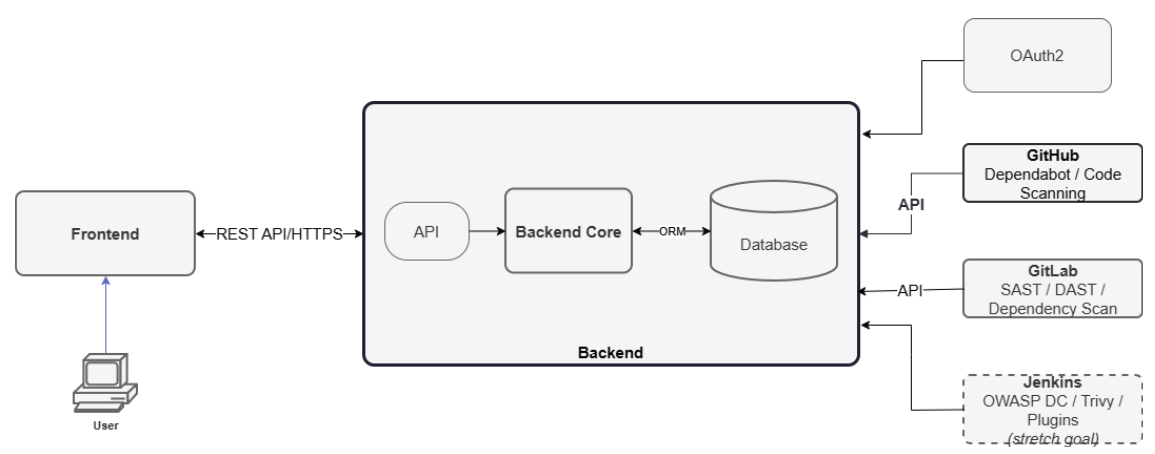
\includegraphics[width=0.75\linewidth]{./figures/diagrama.png}
	\caption{caption teste}
\end{figure}

O \textit{backend} é o principal responsável pela lógica de negócio da aplicação, recaindo nele as funções de comunicar com as APIs externas às quais a aplicação necessita de recorrer e de normalizar a informação recebida destas. É também sua responsabilidade toda a lógica de registo e autorização dos utilizadores e a persistências dos dados numa base de dados. O \textit{backend} atua também como uma \textbf{API REST}, expondo os dados necessários de forma estruturada via pedidos \textbf{HTTP}. \\

Enquanto isso, o \textit{frontend} constitui a interface visual com que o utilizador interage via web browser. O seu papel é consumir os dados enviados pelo \textit{backend} e exibí-los ao utilizador de forma interativa através de uma página web, tratando de toda a lógica de navegação e visualização. \\

Esta separação modular, tendo por base o princípio de \textit{separation of concerns}, para além de permitir escolhas técnicas mais especializadas para cada módulo, reduz a complexidade ao limitar a interação entre estes, permitindo que cada camada evolua de forma independente, facilitando a manutenção e atualização futura do sistema. \\

Para além disso, separar a lógica de apresentação da lógica de dados permite que uma única API, implementada no \textit{backend} venha a servir potenciais múltiplas plataformas (web, desktop, mobile, etc). \\


\section{APIs externas} \label{arquitetura:apis}
O funcionamento da aplicação está intrinsecamente ligado ao usp de APIs externas.  Os utilizadores podem-se autenticar através da utilização do protocolo \textit{OAuth 2.0} usando como \textit{identity providers} Google, GitHub ou GitLab. \\

Estes dois últimos provedores de identidade cumprem um papel duplo, pois para além da possibilidade de providenciarem \textit{autenticação} ao SecDash são também eles que providenciam \textit{autorização}, de forma a que a aplicação possa requisitar os repositórios dos utilizadores bem como consumir os endpoints de segurança que contêm os relatórios de vulnerabilidades sobre os quais a funcionalidade base do projeto assenta. \\

\section{Tecnologias e linguagens} \label{arquitetura:tecnologias}
\subsection{Backend} \label{arquitetura:tecnologias:backend}
\subsection{Frontend} \label{arquitetura:tecnologias:frontend}

% Capitulo 3
\chapter{Implementação} \label{cap:implementacao}

Para facilitar a manutenção e implementação do sistema, bem como a sua compreesão,o \textbf{SecDash} encontra-se decomposto em camadas, seguindo um padrão de desenho \textit{multi-tier} ou \textit{layered}. \\

A aplicação encontra-se dividida em três níveis, numa estrutura hierárquica, sendo estes a \textbf{camada de apresentação}, a \textbf{camada lógica} e a \textbf{camada de dados}. \\

\begin{itemize}
	\item A \textbf{camada de apresentação} tem como função principal ser a interface com a qual o utilizador interage com o \textbf{SecDash}, isto é, o nosso \textit{frontend} web;

	\item A \textbf{camada lógica} é o cerne do programa, tratando-se do nosso backend em kotlin onde é implementada toda a lógica de negócio;

	\item A \textbf{camada de dados} persiste os dados a serem armazenados permanentemente, estando esta implementada como uma base de dados PostgreSQL; 
\end{itemize}

Os detalhes e especifidades da implementação e desenvolvimeto de cada uma destas camadas serão explorados ao longo deste capítulo. \\

\section{Modelo de dados} \label{implementacao:modelo}
A elaboração de um modelo Entidade-Associação é indispensável para a estruturação lógica do projeto. Com efeito, é a existência de um modelo entidade-associação que permite estruturar de forma concreta as entidades do domínio da aplicação e as suas relações entre si. \\

O modelo de dados serve também de ponte entre os requisitos de negócio da plataforma e a sua implementação física na base de dados. Este mapeamento garante que a existência uma visão clara de como os utilizadores, repositórios e vulnerabilidades se relacionam entre si, permitindo orientar a implementação lógica do sistema prevenindo assim o aparecimento de inconsistências estruturais que pudessem pôr em causa a robustez da aplicação ou atrasar o seu desenvolvimento. \\

Como referido no capítulo anterior, os dados obtidos das APIs externas do GitHub e GitLab são altamente estruturados e com dependências e relações claras entre si. Assim sendo, a elaboração de um modelo Entidade-Associação, indispensável para a estruturação lógica do projeto, torna-se relativamente trivial. \\

O diagrama do modelo obtido encontra-se apresentado na figura abaixo. É importante salientar que, de forma a facilitar a apresentação e visualização do modelo no presente documento, os atributos das entidades, bem como a cardinalidade das suas relações, foram omitidos do diagrama. O script SQL utilizado para criar todo o esquema da base de dados, onde se pode consultar todos os atributos, encontra-se no Apêndice \ref{ap:schema}. \\

\begin{figure}[h]
	\centering
	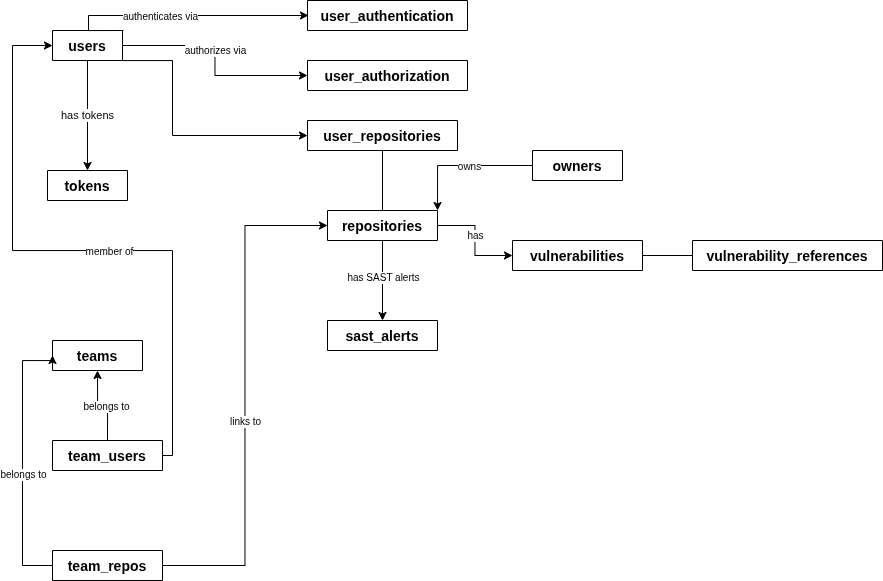
\includegraphics[width=0.95\linewidth]{./figures/secdash-ea.drawio.png}
	\caption{diagrama do modelo de dados}
\end{figure}

\begin{itemize}
	\item Cada \textbf{USER} possui um \textbf{id} que os identificará na aplicação, bem como um \textbf{name} e \textbf{email}. Poderão também ter um campo \textit{\textbf{password\_validation}}, opcional, caso optem por se registar na aplicação diretamente com o seu email em vez de utilizarem uma das opções OAuth 2.0. \\
	
	Cada user terá também uma \textit{\textbf{role}}, que o identificará como um utilizador normal ou administrador, tendo este último acesso a funcionalidades vedadas a utilizadores normais, tais como eliminar utilizadores ou equipas que não lhe pertencem. \\
	
	As informações de autenticação são guardadas na tabela \textbf{USER\_AUTHENTICATION}, que irá conter os IDs de cada utilizador, o provedor de autenticação OAuth 2.0  (Google, GitHub ou GitLab) e o ID do utilizador nessa plataforma. \\
	
 	Os \textit{access tokens} de cada utilizador ficam armazenados na tabela \textbf{USER\_AUTHORIZATION}. Os \textit{tokens} internos gerados e usados pelo próprio \textbf{SecDash}, por sua vez, são armazedados na tabela \textbf{TOKENS}. \\
	
	\item Cada repositório vigiado pela aplicação é armazenado na tabela \textbf{REPOSITORIES}. A tabela \textbf{OWNERS} armazena algumas informações referentes aos proprietários dos repositórios nas plataformas de origem, seja ela GitHub ou GitLab. Para fazer a ligação entre os repositórios armazenados e os utilizadores que os vigiam existe a tabela \textbf{USER\_REPOSITORIES}. \\ 
	
	Os alertas SAST e vulnerabilidades detetadas nas dependências de cada repositório são armazenados nas tabelas \textbf{SAST\_ALERTS} e \textbf{VULNERABILITIES} respetivamente. Esta última tabela encontra-se também ligada à tabela \textbf{VULNERABILITY\_REFERENCES}, que armazena ligações as CVEs onde essas vulnerabilidades estão catalogadas. \\
	
	\item Finalmente, as informações de cada equipa criada no âmbito da aplicação são armazenadas da tabela \textbf{TEAMS}. Os repositórios e utilizadores ligados a cada uma são armazenados nas tabelas \textbf{TEAM\_REPOS} e \textbf{TEAM\_USERS} respetivamente. \\
\end{itemize}

É importante indicar que ao obter os dados das APIs externas, sejam estes referentes a repositórios ou vulnerabilidades, a informação devolvida contém inúmeros campos que não consideramos relevantes de armazenar ou exibir aos utilizadores para os propósitos do \textbf{SecDash}. A título de exemplo, o objeto JSON referente a um repoisitório GitHub devolvido pela sua API contém mais de 80 campos, sendo vários deles objetos que por sua vez contém também múltiplos campos. Um exemplo deste formato pode ser consultado no Apêndice \ref{ap:repogithub}. Como tal, optou-se por filtrar muitos destes campos, sendo apenas armazenados aqueles que considerámos relevantes para o propósito da aplicação.

\section{Backend} \label{implementacao:backend}
O \textit{backend} do \textbf{SecDash} encontra-se estruturado com o padrão de desenho \textbf{Controller-Service-Repository (CSR)}. Pretende-se deste modo isolar o tratamento de pedidos HTTP, a lógica de negócio e operações de base de dados em componentes independentes. Organizar a aplicação desta forma tem o intuito de facilitar o seu desenvolvimento e manutenção. \\

\subsection{Controllers}
A camada dos \textit{controllers} tem como principal objetivo receber pedidos HTTP para consequentemente devolver respostas HTTP. A camada conta com cinco controllers distintos, cada um com endpoints próprios para cada operação suportada pela aplicação: 
\begin{itemize}
	\item \textbf{Auth Controller:} Responsável por receber pedidos HTTP relacionados com autorização externa , tais como pedidos de \textit{login} através de OAuth 2.0 na aplicação ou conceder acesso aos repositórios de um utilizador de uma das plataformas externas;
	
	\item \textbf{GitHub Controller:} Responsável por receber pedidos e emitir as respetivas respostas para tarefas que requiram acesso ao GitHub, tais como adicionar um repositório do GitHub aos repositórios vigiados pelo utilizador com sessão ativa, ou obter análises de vulnerabilidade de um desses repositórios;
	
	\item \textbf{GitLab Controller:} Análogo ao controller anterior mas para GitLab;
	
	\item \textbf{Repo Controller:} Responsável por receber e responder a pedidos HTTP relacionados com os repositórios inseridos no domínio do \textbf{SecDash};
	
	\item \textbf{Team Controller:} Responsável por receber pedidos HTTP e emitir as respetivas respostas para operações relacionadas com equipas no \textbf{SecDash}. Os utilizadores podem criar ou eliminar equipas, adicionar ou remover repositórios e outros utilizadores a equipas ou promover membros de uma equipa a Team Leader;
	
	\item \textbf{User Controller:} Responsável por receber e responder a pedidos HTTP para registo na aplicação através do formulário de registo ou de obter informação do utilizador com sessão ativa;
	
\end{itemize}

Para manter o isolamento das camadas, nenhuma lógica de negócio ou processamento de dados é executado nesta camada. Esse tipo de tarefas é delegado para a camada dos serviços, que será detalhada na subseção seguinte. Não obstante, para efeitos de organização do código, optou-se por colocar alguns componentes necessários para uma utilização mais eficiente da \textit{framerwork} Spring e evitar repetição de código numa subpackage entitulada \textit{pipeline} na \textit{package} dos controllers. Estes componentes encontram-se explicitados na subsecção Pipeline. \\

\subsection{Pipeline}

\begin{table}[htbp]
	\centering
	\caption{Responsabilidades dos componentes do pipeline de execução no Backend.}
	\label{tab:pipeline_components}
	\begin{tabular}{|l|p{10cm}|}
		\hline
		\textbf{Componente} & \textbf{Breve Descrição da Responsabilidade} \\ \hline
		\texttt{AuthenticatedUserArgumentResolver} & Injeta automaticamente o objeto \texttt{AuthenticatedUser} nos parâmetros dos \textit{controllers} que requerem a identidade do utilizador. \\ \hline
		\texttt{AuthenticationInterceptor} & Interceta os pedidos ao nível do Spring MVC para validar o \textit{token} (\textit{header} ou \textit{cookie}) antes que estes atinjam os endpoints protegidos. \\ \hline
		\texttt{BearerTokenAuthFilter} & Filtro de baixo nível que valida as credenciais do utilizador e integra a sessão ativa no contexto global de segurança do Spring Security. \\ \hline
		\texttt{GlobalExceptionHandler} & Centraliza a captura de erros não tratados na API, transformando exceções inesperadas em respostas formatadas e seguras para o cliente. \\ \hline
		\texttt{OAuthRedirectFilter} & Preserva e armazena na sessão o URI de redirecionamento original do utilizador durante o início do fluxo de autenticação por OAuth2.0. \\ \hline
		\texttt{RequestTokenProcessor} & Abstrai a lógica de extração, parsing e validação de \textit{tokens}, gerindo também a criação e destruição de \textit{cookies} seguros. \\ \hline
	\end{tabular}
\end{table}

\subsection{Services}
A camada dos serviços é onde se processa a lógica de negócio da aplicação. Esta camada está organizada de forma semelhante à camada de \textit{controllers} já descrita, com a separação em cinco serviços distintos. \\

Um dos detalhes que vale a pena realçar é o uso que cada um dos serviços faz de uma classe que lhe é injetada com o nome de \textbf{transactionManager}. Trata-se de uma classe implementada com o nome \textbf{JdbiTransactionManager} e tem o propósito de gerir a execução de operações à base de dados dentro de transações na camada de serviços, utilizando a biblioteca JDBI, para que não seja esta camada a ter de liderar diretamente com a abertura, commit ou rollback de transações. \\

Tal é feito através do método \textit{inTransaction} da JDBI, que recebe um bloco de código e executa-a dentro de uma transação controlada por essa biblioteca. Se a execução do bloco for bem-sucedida a transação é confirmada automaticamente. Caso contrário, é feito o \textit{rollback} também automaticamente. \\

\subsection{Repositories e REST Clients}
Nesta camada é onde se processa o acesso à base de dados e a APIs externas. \\

A package \textbf{restclient} contém as classes \textbf{GitHubRestClient} e \textbf{GitLabRestClient} onde, através do RestClient nativo do Spring, fazemos as chamadas a estas APIs. A \textit{package} \textbf{repository} contém as classes onde é acedida a base de dados através de transações JDBI. \\

Devido à hetereogeneidade dos dados, em muitas transações é necessário mapear o \textit{Result Set} obtido através do uso de \textit{Data Transfer Objects} (DTOs) por nós implementados. Estes encontram-se na \textit{pacakage} \textbf{model}, junto às respetivas classes de destino. \\

\subsection{Security Config}
A classe \textbf{SecurityConfig} é responsável pela configuração global da segurança da aplicação através do \textbf{Spring Security}. É através desta classe que são definidos como os pedidos HTTP são autenticados, que endpoints são de acesso público ou protegidos e a integração de mecanismos de autenticação. \\

A anotação \textbf{@EnableWebSecurity} ativa o suporte ao \textbf{Spring Security}, permitindo a definição de regras de autenticação e autorização, bem como a integração com mecanismos como filtros personalizados e com o protocolo \textbf{OAuth2.0}. \\

Os métodos anotados com \textbf{@Bean} são registados no contexto do Spring como beans por ele geridos, permitindo assim que componentes como o \textbf{SecurityFilterChain} e o \textbf{AuthenticationSuccessHandler} sejam instanciados e geridos automaticamente pela framework e injetados onde necessário. Sem esse registo no \textit{startup} da aplicação não seria possível integrar a lógica de autenticação por nós desenvolvida com recurso ao \textbf{BearerTokenAuthFilter} e ao \textbf{OAuthRedirectFilter} anteriormente discutidos no presente capítulo. \\

\section{Frontend} \label{implementacao:frontend}
A arquitetura do cliente web foi desenvolvida recorrendo à biblioteca \textbf{React}, com um foco na modularidade e reatividade da interface de utilizador. \\

O cliente segue uma estrutura \textit{Single Page Application}(SPA) onde inicialmente é carregada uma única página base cujo conteúdo é atualizado dinamicamente em resposta às ações do utilizador. É assim garantida uma experiência de utilização fluida e desacoplada, com o browser do navegador a comunicar de forma assíncrona com a API do \textit{backend} através de pedidos HTTP. \\

As subsecções seguintes abordam alguns elementos do cliente Web que julgamos merecerem algum em destaque. \\

\subsubsection{RequireAuthentication}

O componente \textbf{RequireAuthentication} tem como responsabilidade intercetar os acessos a qualquer URI da aplicação que exija que o utilizador tenha sessão iniciada para que a presença de uma sessão ativa possa ser validada antes de os componentes serem exibidos. Ao tentar aceder a uma rota protegida, caso o utilizador não possua um token válido, este será automaticamente redirecionado para a página de login. \\

\subsubsection{ThemeProvider}

O \textbf{ThemeProvider} é o componente responsável por gerir e persistir o esquema de cores da aplicação, contanto com dois temas: escuro e claro. \\

É garantida uma experiência visual consistente ao longo de toda a \textit{Single Page Application}. Para evitar o efeito visual desagradável de possivelmente carregar inicialmente o tema claro e só depois ser carregado o escuro que um utilizador tenha ativado ao mudar de página, o estado inicial do tema é determinado através de uma função de iniciação \textit{lazy} no \textbf{useState}, que verifica qual o tema selecionado pelo utilizador, armazenado no \textit{localStorage}. \\

O tema atual é disponibilizado a todo o frontend através do \textbf{ThemeContext}. \\

\subsection{i18n}

O frontend do \textbf{SecDash} foi implementado tendo em vista a possibilidade de exibir uma interface com várias línguas distintas. \\

A lógica de implementação desta funcionalidade está centrada no componente \textbf{I18nProvider}, que recorre à \textit{Context API} do React para armazenar o idioma ativo (\textit{Locale}) e expor o seu dicionário de traduções. \\


% Capitulo 4
\chapter{Deployment} \label{cap:deployment}


% Capitulo 5
\chapter{Dificuldades Técnicas e teóricas} \label{cap:dificuldades}

% Capitulo 6
\chapter{Conclusão} \label{cap:conclusao}
\section{Dificuldades Técnicas e teóricas} \label{cap:dificuldades}
\section{Considerações finais}

% Referências
\bibliographystyle{unsrt}
\bibliography{referencias}
\addcontentsline{toc}{chapter}{Refer\^{e}ncias}

% Apêndices (opcional)
\appendix
%
% Apêndice 1
%
\chapter{Exemplo do formato de resposta JSON de um repositório GitHub} \label{ap:repogithub}
\begin{lstlisting}
	 {
		"id": 735375108,
		"node_id": "R_kgDOK9TvBA",
		"name": "IPW-FINAL",
		"full_name": "gfdcarvalho/IPW-FINAL",
		"private": true,
		"owner": {
			"login": "gfdcarvalho",
			"id": 87329708,
			"node_id": "MDQ6VXNlcjg3MzI5NzA4",
			"avatar_url": "https://avatars.githubusercontent.com/u/87329708?v=4",
			"gravatar_id": "",
			"url": "https://api.github.com/users/gfdcarvalho",
			"html_url": "https://github.com/gfdcarvalho",
			"followers_url": "https://api.github.com/users/gfdcarvalho/followers",
			"following_url": "https://api.github.com/users/gfdcarvalho/following{/other_user}",
			"gists_url": "https://api.github.com/users/gfdcarvalho/gists{/gist_id}",
			"starred_url": "https://api.github.com/users/gfdcarvalho/starred{/owner}{/repo}",
			"subscriptions_url": "https://api.github.com/users/gfdcarvalho/subscriptions",
			"organizations_url": "https://api.github.com/users/gfdcarvalho/orgs",
			"repos_url": "https://api.github.com/users/gfdcarvalho/repos",
			"events_url": "https://api.github.com/users/gfdcarvalho/events{/privacy}",
			"received_events_url": "https://api.github.com/users/gfdcarvalho/received_events",
			"type": "User",
			"user_view_type": "public",
			"site_admin": false
		},
		"html_url": "https://github.com/gfdcarvalho/IPW-FINAL",
		"description": null,
		"fork": false,
		"url": "https://api.github.com/repos/gfdcarvalho/IPW-FINAL",
		"forks_url": "https://api.github.com/repos/gfdcarvalho/IPW-FINAL/forks",
		"keys_url": "https://api.github.com/repos/gfdcarvalho/IPW-FINAL/keys{/key_id}",
		"collaborators_url": "https://api.github.com/repos/gfdcarvalho/IPW-FINAL/collaborators{/collaborator}",
		"teams_url": "https://api.github.com/repos/gfdcarvalho/IPW-FINAL/teams",
		"hooks_url": "https://api.github.com/repos/gfdcarvalho/IPW-FINAL/hooks",
		"issue_events_url": "https://api.github.com/repos/gfdcarvalho/IPW-FINAL/issues/events{/number}",
		"events_url": "https://api.github.com/repos/gfdcarvalho/IPW-FINAL/events",
		"assignees_url": "https://api.github.com/repos/gfdcarvalho/IPW-FINAL/assignees{/user}",
		"branches_url": "https://api.github.com/repos/gfdcarvalho/IPW-FINAL/branches{/branch}",
		"tags_url": "https://api.github.com/repos/gfdcarvalho/IPW-FINAL/tags",
		"blobs_url": "https://api.github.com/repos/gfdcarvalho/IPW-FINAL/git/blobs{/sha}",
		"git_tags_url": "https://api.github.com/repos/gfdcarvalho/IPW-FINAL/git/tags{/sha}",
		"git_refs_url": "https://api.github.com/repos/gfdcarvalho/IPW-FINAL/git/refs{/sha}",
		"trees_url": "https://api.github.com/repos/gfdcarvalho/IPW-FINAL/git/trees{/sha}",
		"statuses_url": "https://api.github.com/repos/gfdcarvalho/IPW-FINAL/statuses/{sha}",
		"languages_url": "https://api.github.com/repos/gfdcarvalho/IPW-FINAL/languages",
		"stargazers_url": "https://api.github.com/repos/gfdcarvalho/IPW-FINAL/stargazers",
		"contributors_url": "https://api.github.com/repos/gfdcarvalho/IPW-FINAL/contributors",
		"subscribers_url": "https://api.github.com/repos/gfdcarvalho/IPW-FINAL/subscribers",
		"subscription_url": "https://api.github.com/repos/gfdcarvalho/IPW-FINAL/subscription",
		"commits_url": "https://api.github.com/repos/gfdcarvalho/IPW-FINAL/commits{/sha}",
		"git_commits_url": "https://api.github.com/repos/gfdcarvalho/IPW-FINAL/git/commits{/sha}",
		"comments_url": "https://api.github.com/repos/gfdcarvalho/IPW-FINAL/comments{/number}",
		"issue_comment_url": "https://api.github.com/repos/gfdcarvalho/IPW-FINAL/issues/comments{/number}",
		"contents_url": "https://api.github.com/repos/gfdcarvalho/IPW-FINAL/contents/{+path}",
		"compare_url": "https://api.github.com/repos/gfdcarvalho/IPW-FINAL/compare/{base}...{head}",
		"merges_url": "https://api.github.com/repos/gfdcarvalho/IPW-FINAL/merges",
		"archive_url": "https://api.github.com/repos/gfdcarvalho/IPW-FINAL/{archive_format}{/ref}",
		"downloads_url": "https://api.github.com/repos/gfdcarvalho/IPW-FINAL/downloads",
		"issues_url": "https://api.github.com/repos/gfdcarvalho/IPW-FINAL/issues{/number}",
		"pulls_url": "https://api.github.com/repos/gfdcarvalho/IPW-FINAL/pulls{/number}",
		"milestones_url": "https://api.github.com/repos/gfdcarvalho/IPW-FINAL/milestones{/number}",
		"notifications_url": "https://api.github.com/repos/gfdcarvalho/IPW-FINAL/notifications{?since,all,participating}",
		"labels_url": "https://api.github.com/repos/gfdcarvalho/IPW-FINAL/labels{/name}",
		"releases_url": "https://api.github.com/repos/gfdcarvalho/IPW-FINAL/releases{/id}",
		"deployments_url": "https://api.github.com/repos/gfdcarvalho/IPW-FINAL/deployments",
		"created_at": "2023-12-24T17:26:14Z",
		"updated_at": "2023-12-24T17:28:00Z",
		"pushed_at": "2023-12-29T00:01:03Z",
		"git_url": "git://github.com/gfdcarvalho/IPW-FINAL.git",
		"ssh_url": "git@github.com:gfdcarvalho/IPW-FINAL.git",
		"clone_url": "https://github.com/gfdcarvalho/IPW-FINAL.git",
		"svn_url": "https://github.com/gfdcarvalho/IPW-FINAL",
		"homepage": null,
		"size": 4045,
		"stargazers_count": 0,
		"watchers_count": 0,
		"language": "JavaScript",
		"has_issues": true,
		"has_projects": true,
		"has_downloads": true,
		"has_wiki": false,
		"has_pages": false,
		"has_discussions": false,
		"forks_count": 0,
		"mirror_url": null,
		"archived": false,
		"disabled": false,
		"open_issues_count": 0,
		"license": null,
		"allow_forking": true,
		"is_template": false,
		"web_commit_signoff_required": false,
		"has_pull_requests": true,
		"pull_request_creation_policy": "all",
		"topics": [],
		"visibility": "private",
		"forks": 0,
		"open_issues": 0,
		"watchers": 0,
		"default_branch": "main",
		"permissions": {
			"admin": false,
			"maintain": false,
			"push": true,
			"triage": true,
			"pull": true
		}
	}
\end{lstlisting}

\chapter{Script SQL para a criação da base de dados} \label{ap:schema}
\begin{lstlisting}[language=SQL, basicstyle=\ttfamily\small, breaklines=true, frame=single, showstringspaces=false, commentstyle=\color{green!50!black}]

	CREATE TYPE platform AS ENUM ('GITHUB', 'GITLAB');
	CREATE TYPE visibility AS ENUM ('PUBLIC', 'PRIVATE', 'INTERNAL');
	CREATE TYPE vulnerability_severity AS ENUM ('CRITICAL', 'HIGH', 'MEDIUM', 'LOW', 'UNKNOWN');
	CREATE TYPE vulnerability_state AS ENUM ('OPEN', 'FIXED', 'DISMISSED');
	CREATE TYPE sast_severity AS ENUM ('CRITICAL', 'HIGH', 'MEDIUM', 'LOW');
	CREATE TYPE sast_state AS ENUM ('OPEN', 'FIXED', 'DISMISSED');
	CREATE TYPE auth_provider AS ENUM ('GOOGLE', 'GITHUB', 'GITLAB');
	CREATE TYPE app_roles as ENUM ('ADMIN', 'USER');
	CREATE TYPE team_roles as ENUM ('LEADER', 'COLLABORATOR');
	
	CREATE TABLE users (
	uid                     INT GENERATED ALWAYS AS IDENTITY PRIMARY KEY,
	name                    VARCHAR(255) NOT NULL,
	password_validation     TEXT,
	email                   VARCHAR(255) NOT NULL UNIQUE,
	role                    app_roles NOT NULL DEFAULT 'USER'
	);
	

	CREATE TABLE user_authentication (
	user_id     INT           NOT NULL REFERENCES users(uid),
	provider    auth_provider NOT NULL,
	provider_id VARCHAR       NOT NULL,
	PRIMARY KEY (user_id, provider),
	UNIQUE      (provider, provider_id)
	);
	

	CREATE TABLE user_authorization (
	user_id      INT           NOT NULL REFERENCES users(uid),
	provider     auth_provider NOT NULL,
	access_token TEXT          NOT NULL,
	PRIMARY KEY  (user_id, provider)
	);
	

	CREATE TABLE tokens (
	token_validation    VARCHAR(256) primary key,
	user_id             int references users(uid),
	created_at          bigint not null,
	last_used_at        bigint not null
	);
	

	CREATE TABLE owners (
	oid             INT GENERATED ALWAYS AS IDENTITY PRIMARY KEY,
	external_id     VARCHAR(255),
	name            VARCHAR(255) NOT NULL,
	url             VARCHAR(255) NOT NULL,
	avatar_url      VARCHAR(255),
	platform        platform     NOT NULL,
	UNIQUE (external_id, platform)
	);
	

	CREATE TABLE repositories (
	rid          INT GENERATED ALWAYS AS IDENTITY PRIMARY KEY,
	name         VARCHAR(255) NOT NULL,
	external_id  VARCHAR(255) NOT NULL,
	platform     platform     NOT NULL,
	owner_id     INT          NOT NULL REFERENCES owners(oid),
	html_url     VARCHAR(255) NOT NULL,
	description  TEXT,
	issues_count INT          NOT NULL DEFAULT 0,
	created_at   TIMESTAMPTZ    NOT NULL,
	updated_at   TIMESTAMPTZ    NOT NULL,
	forks_count  INT          NOT NULL DEFAULT 0,
	visibility   visibility   NOT NULL,
	UNIQUE  (external_id, platform)
	);
	

	CREATE TABLE vulnerabilities (
	vid                      INT GENERATED ALWAYS AS IDENTITY PRIMARY KEY,
	external_id              VARCHAR(255)           NOT NULL,
	title                    VARCHAR(255)           NOT NULL,
	description              TEXT,
	severity                 vulnerability_severity NOT NULL,
	state                    vulnerability_state    NOT NULL,
	cve_id                   VARCHAR(50),
	ghsa_id                  VARCHAR(50),
	package_name             VARCHAR(255)           NOT NULL,
	package_version          VARCHAR(100),
	vulnerable_version_range VARCHAR(255),
	fixed_version            VARCHAR(100),
	manifest_path            VARCHAR(255),
	cvss_score               DOUBLE PRECISION,
	cvss_vector              VARCHAR(255),
	platform                 platform               NOT NULL,
	rid                      INT                    NOT NULL REFERENCES repositories(rid),
	detected_at              TIMESTAMP              NOT NULL,
	updated_at               TIMESTAMP              NOT NULL
	);
	

	CREATE TABLE vulnerability_references (
	id      INT GENERATED ALWAYS AS IDENTITY PRIMARY KEY,
	vuln_id INT  NOT NULL REFERENCES vulnerabilities(vid),
	url     TEXT NOT NULL
	);
	

	CREATE TABLE user_repositories (
	uid INT NOT NULL REFERENCES users(uid),
	rid INT NOT NULL REFERENCES repositories(rid),
	PRIMARY KEY (uid, rid)
	);
	

	CREATE TABLE sast_alerts (
	sid        INT GENERATED ALWAYS AS IDENTITY PRIMARY KEY,
	rid        INT           NOT NULL REFERENCES repositories(rid),
	state      sast_state    NOT NULL,
	severity   sast_severity NOT NULL,
	scanner    VARCHAR(255)  NOT NULL,
	file       VARCHAR(255)  NOT NULL,
	line       VARCHAR(50)   NOT NULL
	);
	
	CREATE TABLE teams (
	tid         INT GENERATED ALWAYS AS IDENTITY PRIMARY KEY,
	name        VARCHAR(255) NOT NULL,
	description TEXT
	);
	
	CREATE TABLE team_users (
	tid     INT NOT NULL REFERENCES teams(tid),
	uid     INT NOT NULL REFERENCES users(uid),
	role    team_roles NOT NULL,
	PRIMARY KEY (tid, uid)
	);
	
	CREATE TABLE team_repos (
	tid     INT NOT NULL REFERENCES teams(tid),
	rid     INT NOT NULL REFERENCES repositories(rid),
	PRIMARY KEY (tid, rid)
	);
\end{lstlisting}

\end{document} 